\section{Photon Detector Simulation}
\label{sec:dp-pds-simulation}

A detailed simulation of the \dshort{pds} response is essential both to compare with data from \dshort{pds} prototypes (see Sec.~\ref{sec:dp-pds-prototypes}) and to validate the \dword{fd} baseline design in terms of its projected performance (see Sec.~\ref{sec:dp-pds-performance}).

%%%%%%%%%%%%%%%%%%%%%%%%%%%%%%%%%%%%%%%%%%%%%%%%%%%%%%%%%%%%%%%%%%%

\subsection{Simulation Framework And Assumptions}
\label{subsec:dp-pds-simulation_assumptions}

The simulation of the \dshort{pds} response is integrated in \dword{larsoft}, the liquid argon software toolkit used by the DUNE Collaboration for simulation and reconstruction. The simulation is divided in three steps: light generation, light propagation and light detection.

For a \dword{mip}, an energy of about \SI{2}{\MeV/\cm} is deposited in \dword{lar}. 
Through decays of excited argon states and ion recombination, about \num{40000} scintillation photons are emitted per \si{\MeV} deposited at null drift field. At the nominal drift field of \SI{500}{\V/\cm}, this amount reduces down to about \num{24000} photons per \si{\MeV} as the recombination process is weaker. 
This signal, known as S1 (see Sec.~\ref{sec:dp-pds-overview}), is common to the single and dual phase technologies.

In the gas layer of the dual phase design, the electrons are amplified through Townsend avalanche in the \dword{lem} holes, and lead to an electroluminescence signal called S2 (see Sec.~\ref{sec:dp-pds-overview}). The electroluminescence gain, $G_{EL}$, i.e. the number of photons produced per electrons crossing the liquid-gas interface, depends on the voltages applied to the \dword{lem}. In our simulations, we typically assume a gain of \SI{300}{photons per extracted electron}. The S1 and S2 signals have similar characteristics in terms of wavelength and time constants. 

Due to different mechanisms during photon propagation (Rayleigh scattering, absorption by impurities in the \lar or by elements constituting the detector), only about a \num{1e-3} fraction of the photons produced in the \lar active volume reaches the \dword{pmt} photo-cathodes. The direct simulation of the large number of photons generated for each track crossing the active volume would require a considerable amount of CPU power and time. Profiting from the fact that the photon emission is isotropic and the detector is uniform and symmetric, it was decided to generate the photon propagation in the detector in a dedicated Geant4 simulation only once, and store the results in a photon library.

The active volume is divided into voxels, and a large amount of photons are isotropically and uniformly generated in every voxel. The amount of photons collected by each \dword{pmt} and the propagation time are stored and later parametrized. For long voxel-\dword{pmt} distances (typically larger than \SI{1}{\m}), a landau function is well suited to reproduce the time distribution. The detection probability, called visibility, the landau parameters (MPV, $\sigma$) and the minimal time needed by the photon to reach the \dword{pmt} are stored in a photon library for all voxel-\dword{pmt} combinations. When a track is generated in the standard \dual \dword{larsoft} simulation toolkit, for each step of the track, the light map is looked up to assign the amount of photons to be collected at each \dword{pmt}, and the arrival time distribution due to the propagation. 

To generate photon libraries, a comprehensive modelling of the geometry for the \dword{wa105}, \dword{pddp} and \dword{dp} \dword{fd} detectors are implemented in GDML files. The GDML files include the main elements that are relevant for light propagation, such as the cathode, the \dword{fc}, the \dwords{lem} and the ground grid. Most detector elements are assumed to be fully absorptive. Thus, when photons reach any of these surfaces, they are removed from the simulation. One exception is \dword{wls} reflector foil surfaces, which are assumed to have \SI{100}{\%} \dshort{wls} efficiency for \SI{127}{\nm} \dshort{lar} light, and a 93\% reflectivity for \SI{430}{\nm} light re-emitted by the wavelength shifter material. In order to quantify the impact of the \dshort{wls} reflector foils for the \dword{dp} \dword{fd} module, three geometries have been tested: no foils, foils entirely covering all four \dword{fc} vertical walls, and foils covering only the upper half of the \dword{fc}. For the \dword{pds} prototypes, no foil geometries have been simulated.

As far as \dword{lar} optical properties are concerned, the simulations assume a \SI{61}{\cm} Rayleigh scattering length and a \SI{20}{\m} absorption length for \SI{127}{\nm} light. The response of the \dword{pmt} is simulated assuming an effective quantum efficiency of \num{0.12} that includes the TPB response of the coated photo-cathode \cite{Bonesini:2018ubd}. A dark count rate of \SI{1.7}{\kilo\hertz} at cryogenic temperature is assumed, as obtained during \dword{pddp} \dword{pmt} calibration \cite{Belver:2018erf}. A linear response of the \dword{pmt} is assumed, multiplying the amount of photons reaching the photo-cathode with the single photo-electron response measured in the laboratory, for a gain of \num{1e7}. In this case, the single-PE response has a time width of \SI{6}{\nano\s}, and an amplitude of \SI{15}{mV}. The digitization of the waveform is simulated considering a sampling rate of \SI{250}{MHz}\footnote{This is the sampling frequency used in the \dshort{wa105} readout, however slower frequencies of \SI{65}{MHz} or \SI{2.5}{MHz} are being considered for the \dword{dp} \dword{pds}.}, \SI{0.5}{mV/ADC} resolution, and an electronics noise of \SI{0.8}{ADC counts RMS} as measured in \dshort{wa105}, see Sec.~\ref{sec:dp-pds-prototypes}. Therefore, the single-PE to baseline noise RMS ratio assumed in the simulations, based on \dshort{wa105} measurements, exceeds \num{30}. 

%%%%%%%%%%%%%%%%%%%%%%%%%%%%%%%%%%%%%%%%%%%%%%%%%%%%%%%%%%%%%%%%%%%

\subsection{Expected Light Yields}
\label{subsec:dp-pds-simulation_yields}

%\begin{dunefigure}[Expected light yield in %\dword{pddp}]{fig:dppd_protodunedp_light_yield}{Expected light yield (in PEs/MeV) in %\dword{pddp} as a function of spatial (x,z) position in the \dword{lar} active volume, %and averaged along the y-axis. In this fiigure, the z-axis is parallel to the drift %direction.}
%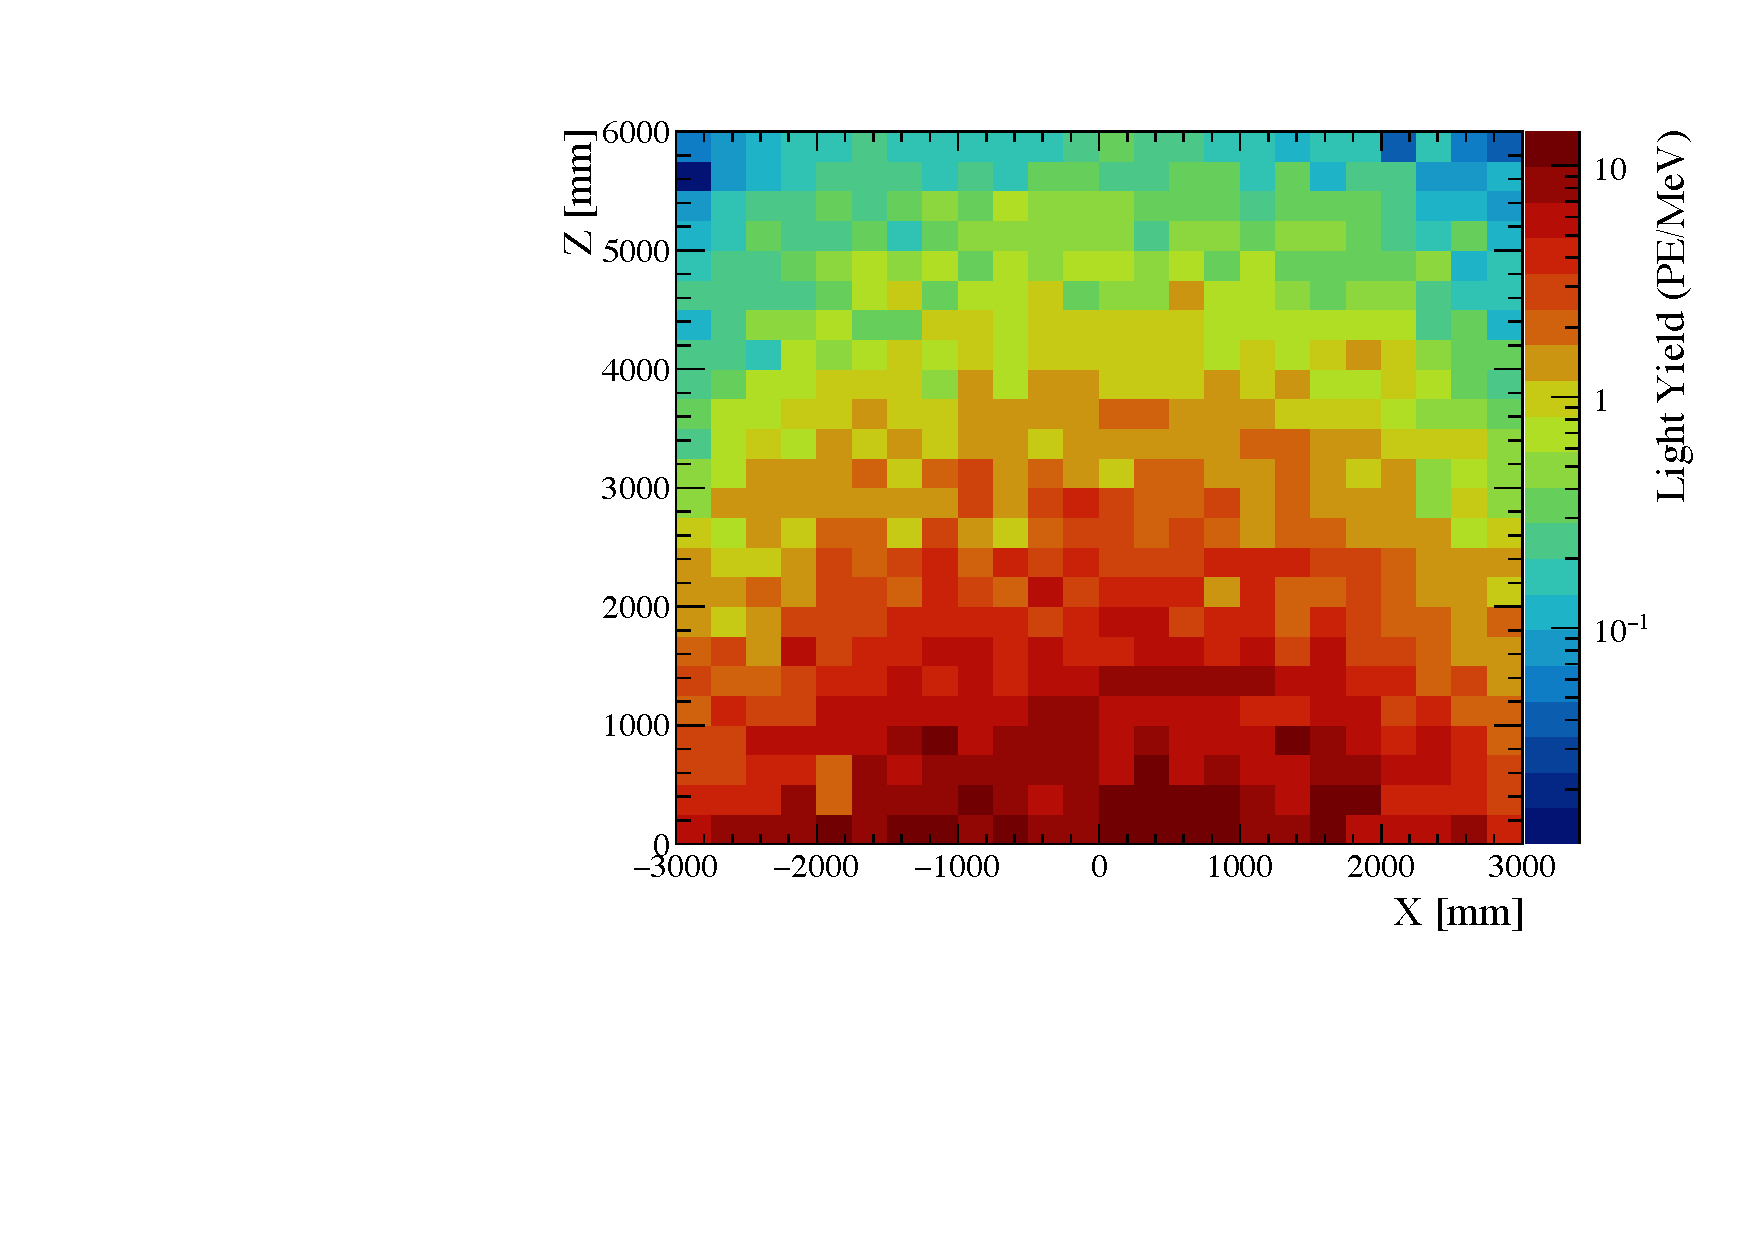
\includegraphics[width=0.6\textwidth]{graphics/dppd_protodunedp_light_yield.pdf}
%\end{dunefigure}

%The \dword{larsoft}-based preliminary photon libraries for the \dword{pddp} and the %\dword{dp} \dword{fd} module geometries have been created. The total light yield per MeV %deposited in \dword{pddp} is shown in Fig.~\ref{fig:dppd_protodunedp_light_yield}. An %average light yield of \SI{2.5}{PEs/MeV} is expected for \dword{pddp}.

Figure~\ref{fig:dppd_fd_light_yield} shows the expected incident light yield, in units of number of photons reaching the \dword{pmt} windows per MeV of deposited energy, and for energy depositions throughout the \dword{dp} \dshort{fd} cryostat. A voxel size of \SI{1}{\m^3} is considered in \dword{dp} \dshort{fd}  simulations. Two geometries are shown: no \dword{wls} reflector foils (left panel of Fig.~\ref{fig:dppd_fd_light_yield}) and foils fully covering \dword{fc} (right panel). In order to obtain the detected light yield, in PEs/\si{MeV} units, the numbers should be multiplied by the effective quantum efficiency of 0.12. The light yields vary over several orders of magnitude, especially along the drift direction and for the no foils case.

\begin{dunefigure}[Expected 2D light yield in the full \dword{dp} \dshort{fd} cryostat.]{fig:dppd_fd_light_yield}
{Expected incident light yield in the full \dword{dp} \dshort{fd} cryostat. The yield units are the number of photons reaching the PMT windows per \si{\MeV} of deposited energy. The 2D yields are shown as a function of the drift direction (along the vertical axis) and of the horizontal direction perpendicular to neutrino beam (along the horizontal axis), averaging over the third spatial coordinate (not shown). The red contours indicate the \dshort{tpc} active volume. Left panel: geometry with no \dword{wls} reflector foils. Right panel: geometry with foils fully covering the \dword{fc}. The \dwords{pmt} are located at a drift coordinate of \SI{-7}{\m}.}
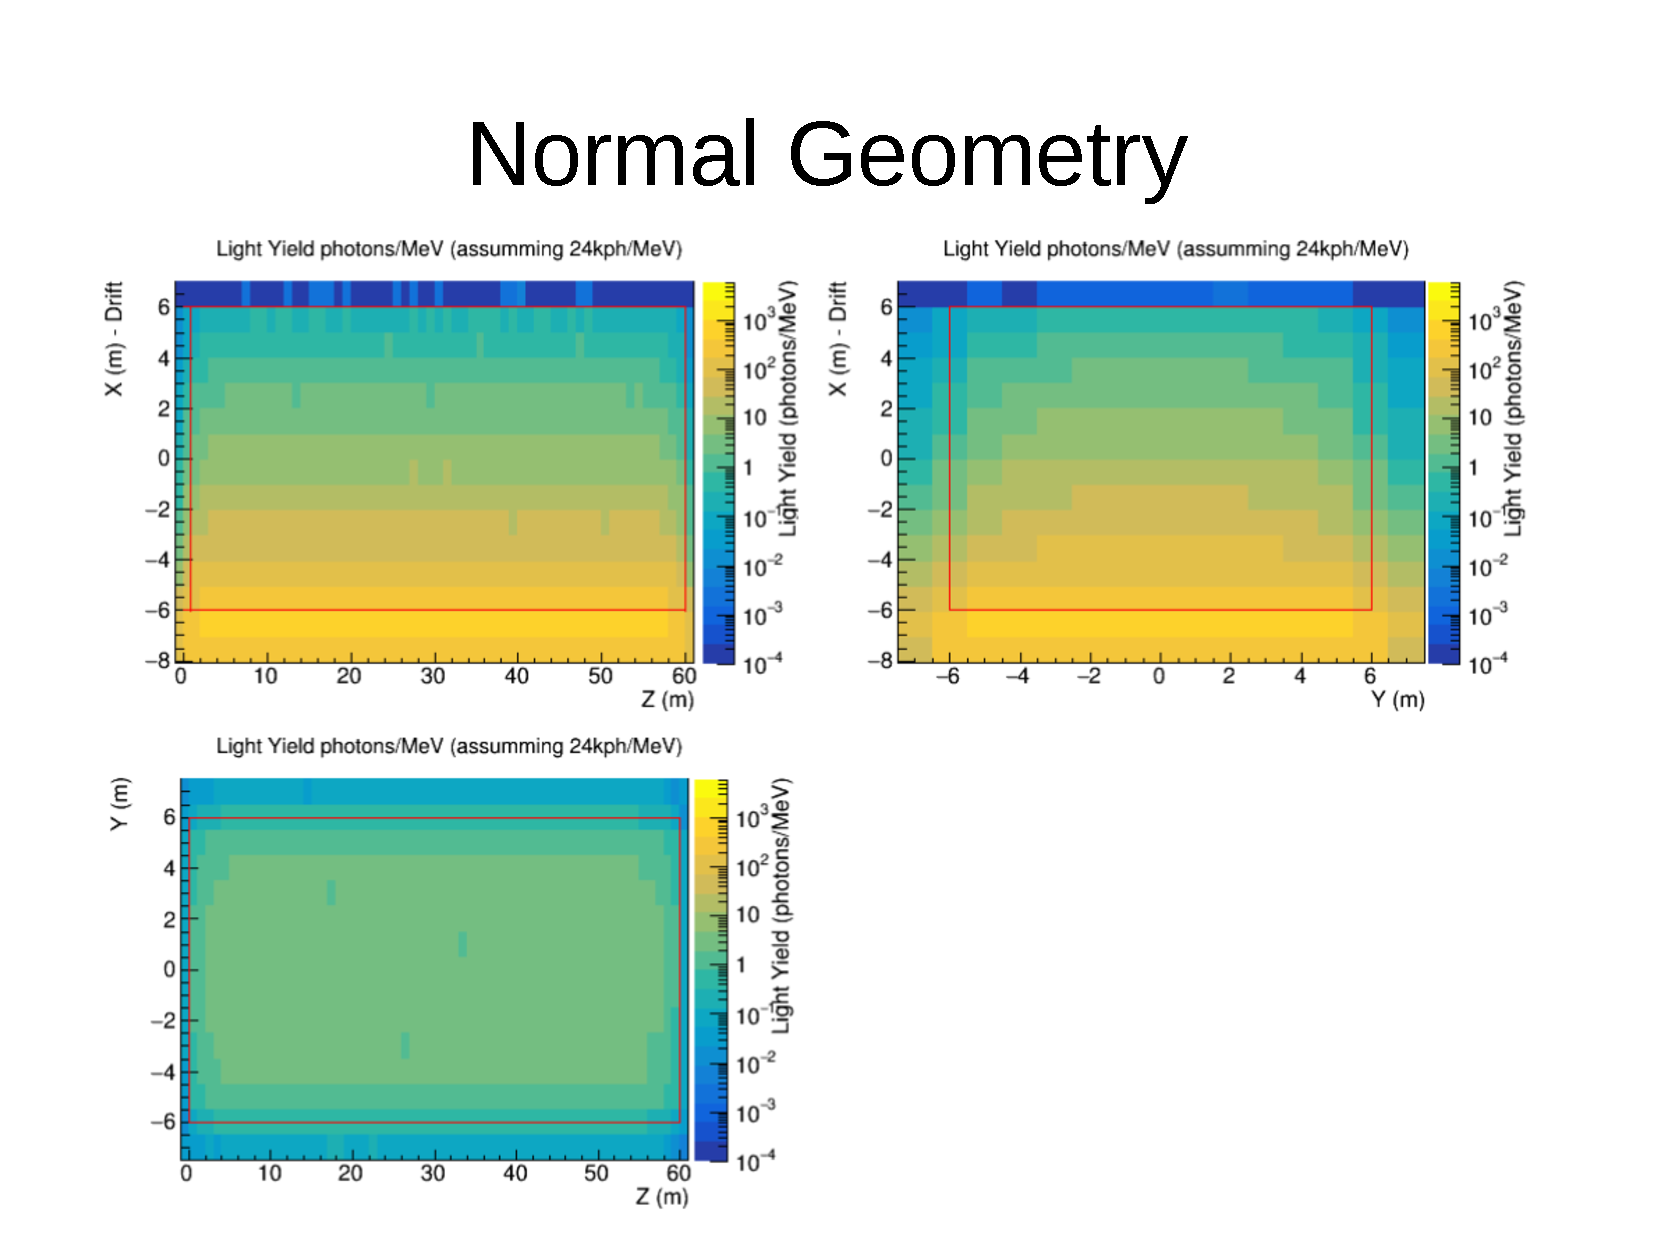
\includegraphics[trim={14cm 9cm 2cm 4.5cm}, clip, height=0.22\textheight]{graphics/dppd_fd_light_yield_nofoil.pdf} \hfill
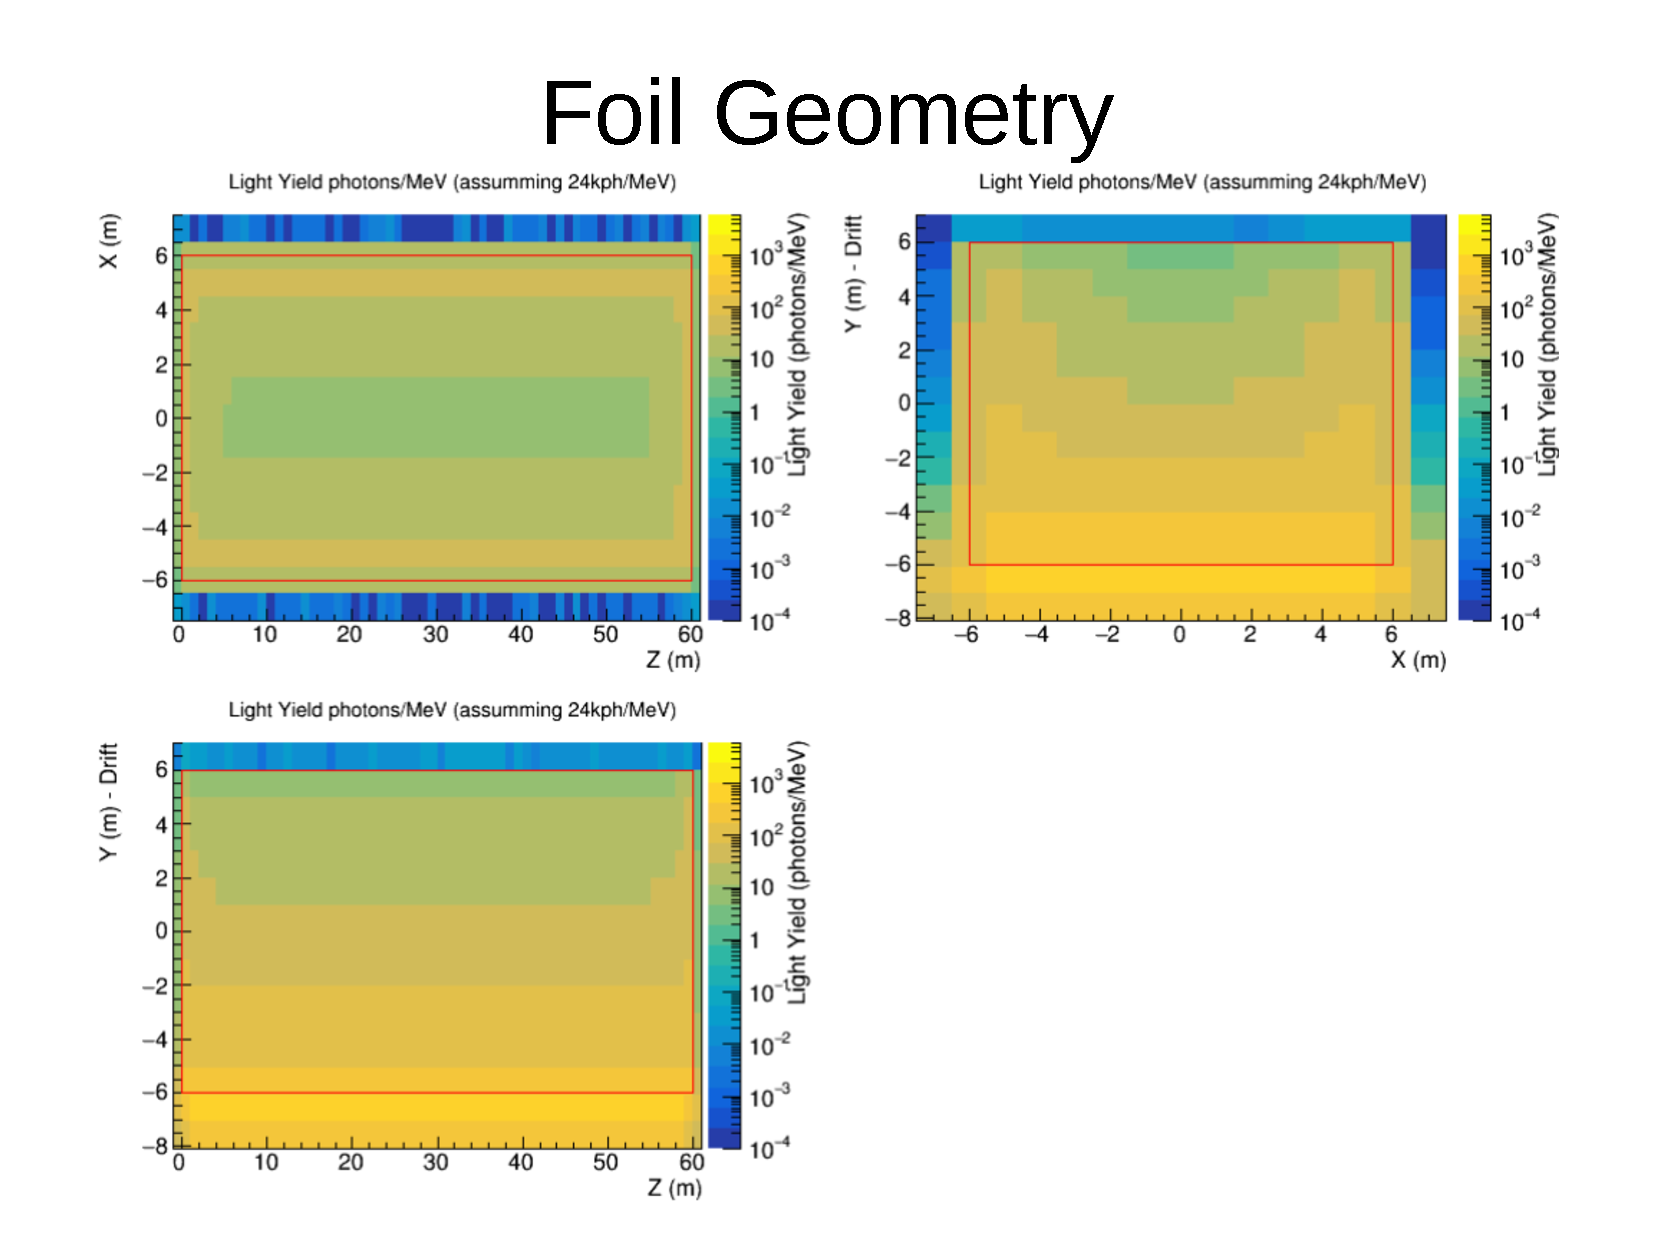
\includegraphics[trim={14cm 9.5cm 1cm 3.5cm}, clip, height=0.22\textheight]{graphics/dppd_fd_light_yield_fullfoil.pdf}
\end{dunefigure}

We can assess the impact of the \dword{wls} reflector foils on the expected light yields more easily in Fig.~\ref{fig:dppd_fd_light_yield_comparison}, where the yields are shown as a function of the drift coordinate only and averaging over the two other spatial coordinates. In this way, one appreciates better the main trend in the spatial response, namely the light yield reduction with increasing distance from the cathode. Three geometries are compared: no foils, foils fully covering the \dword{fc}, foils covering the upper \dword{fc} half. With an average light yield of \SI{5.6}{PEs/MeV}, fully covering the \dword{fc} with \dword{wls} reflector foils is expected to almost double the average light yield compared to the no-foils case, at \SI{3.0}{PEs/MeV}. More importantly, the foils reduce the (very large) non-uniformity in spatial response between cathode and anode by more than one order of magnitude. The option of foils in the upper half of the \dword{fc} only is expected to perform somewhere in between these two scenarios, but closer to the full-foils case.

\begin{dunefigure}[Expected 1D light yield in the full \dword{dp} \dshort{fd} cryostat.]{fig:dppd_fd_light_yield_comparison}
{Expected incident light yield in the full \dword{dp} \dshort{fd} cryostat. The yield units are the number of photons reaching the PMT windows per \si{\MeV} of deposited energy. The 1D yields are shown as a function of the drift direction, averaging over the other two spatial coordinates (not shown). The three histograms correspond to three different geometries: no \dword{wls} reflector foils, foils fully covering \dword{fc}, foils covering upper \dword{fc} half.}
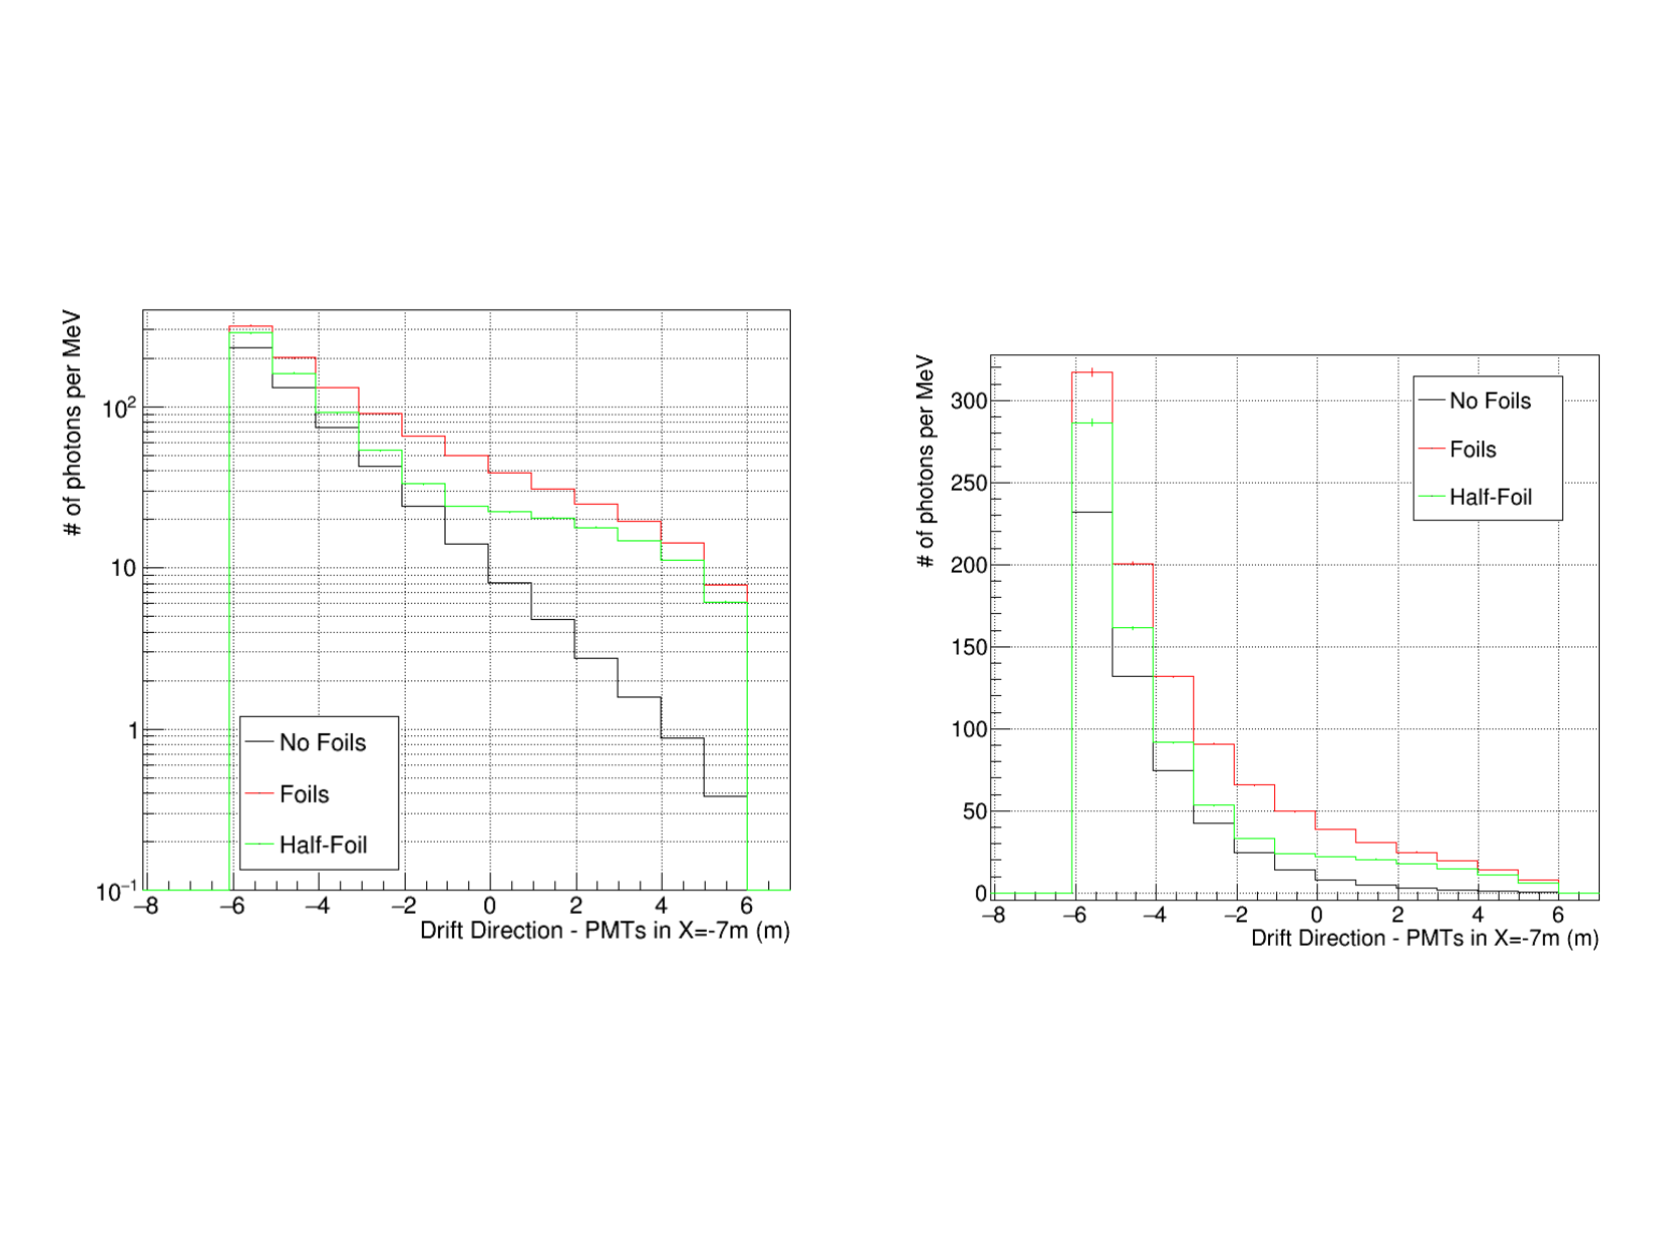
\includegraphics[trim={0cm 5.cm 14cm 5.cm}, clip, width=0.45\textwidth]{graphics/dppd_fd_light_yield_comparison.pdf}
\end{dunefigure}

\fixme{Repeat Figs.~\ref{fig:dppd_fd_light_yield} and \ref{fig:dppd_fd_light_yield_comparison} in PEs/MeV units rather than (incident photons)/MeV units, accounting for different \dshort{pmt} QE for \dshort{lar} and \dshort{wls} light.}